\subsection{Feature selection}
    Una primera idea a la hora de elegir los features de nuestro modelo, es considerar todas las combinaciones posibles de elementos del conjunto de features. Es decir, si el conjunto de features tiene $p$ elementos, consideramos los $p$ modelos con un único feature, luego, consideramos los $\binom{p}{2}$ modelos con dos predictores, y así sucesivamente. El problema con este método es que, la cantidad de modelos a comparar aumenta exponencialmente con el número de features, exactamente, si $p$ es el número de features, entonces  la cantidad de modelos a comparar es $\sum_{k=0}^{p}\binom{p}{k} = 2^p$. Un método menos exacto pero más conservador con respecto a la cantidad de modelos a comparar es el que se conoce como \fss, que pasaremos a explicar a continuación.

\subsubsection{Forward stepwise selection}
    Como mencionamos antes, quisiéramos una manera de seleccionar un modelo, relativamente competente, sin necesidad de clasificar todo el universo de modelos con hasta $p$ features, que como vimos anteriormente, consiste de $2^p$ elementos. La idea de este método es obtener modelos de forma iterativa, y en particular agregativa. El método consiste en ir agregando features, de a una por vez, a un modelo anterior, y eligiendo aquella que mayor impacto tenga en el rendimiento del modelo, este proceso se repite, considerando este nuevo modelo, como el modelo anterior a agregarse features. Formalmente, el método esta definido por el siguiente algoritmo \cite{islr}.
    
    
    \begin{algorithm}[H]
    \begin{enumerate}
        \item Sea $\mathcal{M}_0$ el modelo sin predictores.
        \item Para $k=0, \dots ,p-1$:
        \begin{enumerate}
            \item Consideremos todos los $p-k$ modelos que añaden un predictor al modelo $\mathcal{M}_k$.
            \item Elegimos el \emph{mejor} de estos $p-k$ modelos, y lo llamamos $\mathcal{M}_{k+1}$. Donde \emph{mejor} está definido como el modelo con mayor precisión respecto a la métrica $R^2$.
        \end{enumerate}
        \item Elegimos el mejor modelo del conjunto de los $\mathcal{M}_0,\dots,\mathcal{M}_p$ usando \cv, con respecto a la métrica $R^2$.
    \end{enumerate}
         \caption{Forward stepwise selection}
    \end{algorithm}

    %\begin{enumerate}
    %    \item Sea $\mathcal{M}_0$ el modelo sin predictores.
    %    \item Para $k=0, \dots ,p-1$:
    %    \begin{enumerate}
    %        \item Consideremos todos los $p-k$ modelos que añaden un predictor %al modelo $\mathcal{M}_k$.
    %        \item Elegimos el \emph{mejor} de estos $p-k$ modelos, y lo llamamos $\mathcal{M}_{k+1}$. Donde \emph{mejor} está definido como el modelo con mayor precisión respecto a la métrica $R^2$.
    %    \end{enumerate}
    %    \item Elegimos el mejor modelo del conjunto de los $\mathcal{M}_0,\dots,\mathcal{M}_p$ usando \emph{cross validation}, con respecto a la métrica $R^2$.
    %\end{enumerate}
    
    No obstante, no es cierto que este método siempre encuentre el mejor modelo posible dadas las features que tenemos a nuestra disposición. Por ejemplo, supongamos un conjunto de muestras que poseen $p = 3$ predictores. Puede suceder que el mejor modelo con una única variable, sea aquel que contiene al predictor $X_1$, mientras que el mejor modelo posible sea aquel que contiene a los predictores $X_2$ y $X_3$. Entonces, el método no podrá obtener el mejor modelo posible ya que, todos los modelos en la selección final del método, tendrán que contener a $X_1$. Esta es la concesión que hacemos al usar este método, a cambio reducimos las comparaciones a realizar a $\sum_{i=1}^{p}i = \frac{p(p+1)}{2}.$
    
\subsubsection{Matriz de correlación}
    
    Cuando se deben elegir las variables o features que se utilizaran en el modelo, se puede optar por distintos criterios. Un criterio es el de observar individualmente a través de un gráfico, la relación entre la variable a predecir y la que se utilizará para describirla. Si bien esto suena razonable, optamos también por observar otro aspecto, las correlaciones entre ellas. 
    
    La correlación entre dos variables $X$ e $Y$ nos indica la dependencia entre ellas, es decir, si existe una relación. El valor de la correlación entre ellas esta acotado entre -1 y 1, donde:
    
    \begin{itemize}
        \item Si el valor es cercano a 1 indica que tienen una relación lineal (correlación), cuando $X$ cambia, $Y$ se incrementa linealmente.
        
        \item Si el valor es cercano a -1 indica que tienen una relación lineal inversa (anticorrelación), cuando $X$ cambia, $Y$ decrementa linealmente.
        
        \item Si el valor es cercano a 0 indica que no hay mucha relación (incorrelación).
        
        \item Si el valor esta en el medio de los anteriores, indica el nivel de relación lineal que hay entre las variables.
    \end{itemize}
    
    Bajo este criterio, podemos decir que, dada una variable que queramos predecir, podemos observar sus correlaciones con las demás, y con eso deducir cuales serán mejores para describirla. Esto se puede analizar mediante una matriz de correlación, como la que se muestra a continuación:
    
    \begin{figure}[H]
        \begin{center}
            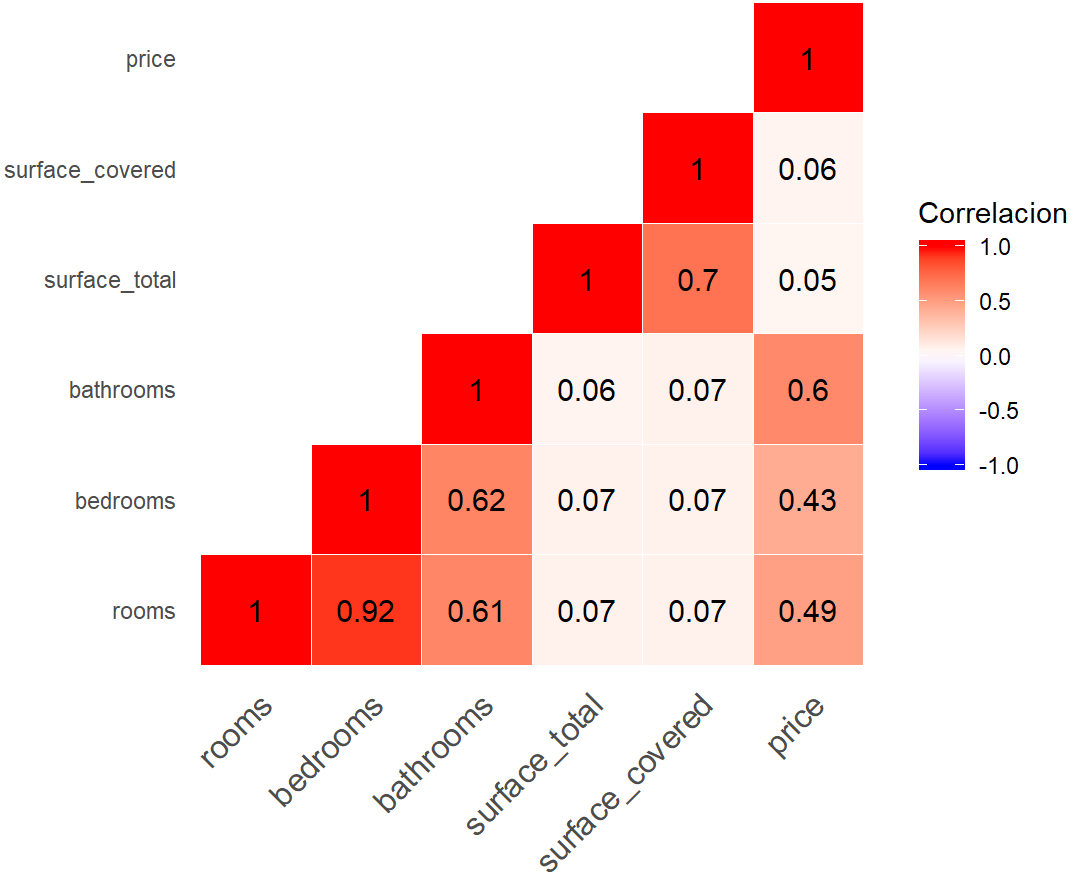
\includegraphics[scale=0.6]{img/explicaciones/Corr-Matrix-Heatmap.png}
            \caption{Matriz de correlación entre características de casas}
            \end{center}
    \end{figure}
    
    En la matriz de la figura anterior, podemos ver la relación de precio con las demás variables. Tenemos por ejemplo, que precio tiene una correlación de 0.49 con habitaciones, 0.43 con dormitorios, y de 0.6 con baños. Esto nos indica que parece buena idea intentar explicar precio con estas 3 variables, sin embargo para metros totales y cubiertos, se tiene 0.05 y 0.06 respectivamente, cercano a 0. Esto ultimo nos indica que no parecen tener relación alguna, y por lo tanto, se puede sospechar que no sean útiles para explicarlo.
    
    Otro punto interesante que nos provee la matriz de correlación, es la relación que hay entre las variables que se quieren utilizar para predecir. Cuando se tienen 2 variables en un modelo que presentan una correlación alta, nos indica que una puede utilizarse para describir a la otra, entonces incluir ambas en el modelo, agregaría redundancia. Por el otro lado, si estas cerca de estar incorrelacionadas, significa que cada una termina aportando información extra a la hora de describir. En el caso del ejemplo anterior, podemos ver que la relación entre dormitorios y habitaciones es de 0.92, lo cual indica que están fuertemente correlacionadas, y es seguro pensar que descartar una de las dos para el modelo final será mejor.
    
    